\documentclass[11pt,titlepage]{article}

%Laenderspezifische Einstellungen bzgl. Rechtschreibung, Sonderzeichen und Kodierung
\usepackage[utf8]{inputenc}
\usepackage[english]{babel}
\usepackage[T1]{fontenc}
\usepackage{titlesec}
\usepackage{graphicx}
\usepackage{subcaption}

\usepackage{listings}
\usepackage{color}
\usepackage{courier}
\definecolor{light-gray}{gray}{0.85}
\lstset{
language=C++,
numbers=left,
breaklines=true,
backgroundcolor=\color{light-gray},
tabsize=2,
basicstyle=\footnotesize\ttfamily,
frame=single,
inputencoding=utf8,
extendedchars=true,
showstringspaces=false,
literate =
	{ä}{{\"a}}1
	{ö}{{\"o}}1
	{ü}{{\"u}}1
	{Ä}{{\"A}}1
	{Ö}{{\"O}}1
	{Ü}{{\"U}}1
	{ß}{{\ss}}1
	{ₙ}{{$_n$}}1
}

\def\ContinueLineNumber{\lstset{firstnumber=last}}

\usepackage[
	a4paper,
	top = 2cm,
	bottom = 2 cm,
	left = 2cm,
	right = 2cm,
	headheight = 15pt,
	includeheadfoot
	]{geometry}
\usepackage{fancyhdr}
\usepackage{amssymb}
\usepackage{amsmath}
\usepackage[english]{varioref}
\usepackage{hyperref}

\fancypagestyle{fancy}{
	\fancyhead[R]{Page \thepage}
	\fancyhead[L]{\leftmark}
	\renewcommand{\headrulewidth}{1.25pt}

	\fancyfoot[L]{\tiny{Algorithms and Data Structures Exercise - Assignment 2, created: \today}}
	\fancyfoot[R]{\tiny{ Felix Dreßler (k12105003)}}
	\cfoot{}
	\renewcommand{\footrulewidth}{1.25pt}
}

\setlength{\headsep}{10mm}
\setlength{\footskip}{10mm}

\setlength{\parindent}{0mm}
\setlength{\parskip}{1.1ex plus0.25ex minus0.25ex}
\setlength{\tabcolsep}{0.2cm} % for the horizontal padding

\pagestyle{fancy}


\begin{document}
	Note: The other Tasks were all done in the Files Main.cpp, Functions.h and Matrix.h. Also all Questions were answered directly in the implementation using comments.
	
	\section{Task 7 - complexity analysis}
	
	Given the complexity analysis of Binary Search from the lecture: 
	
	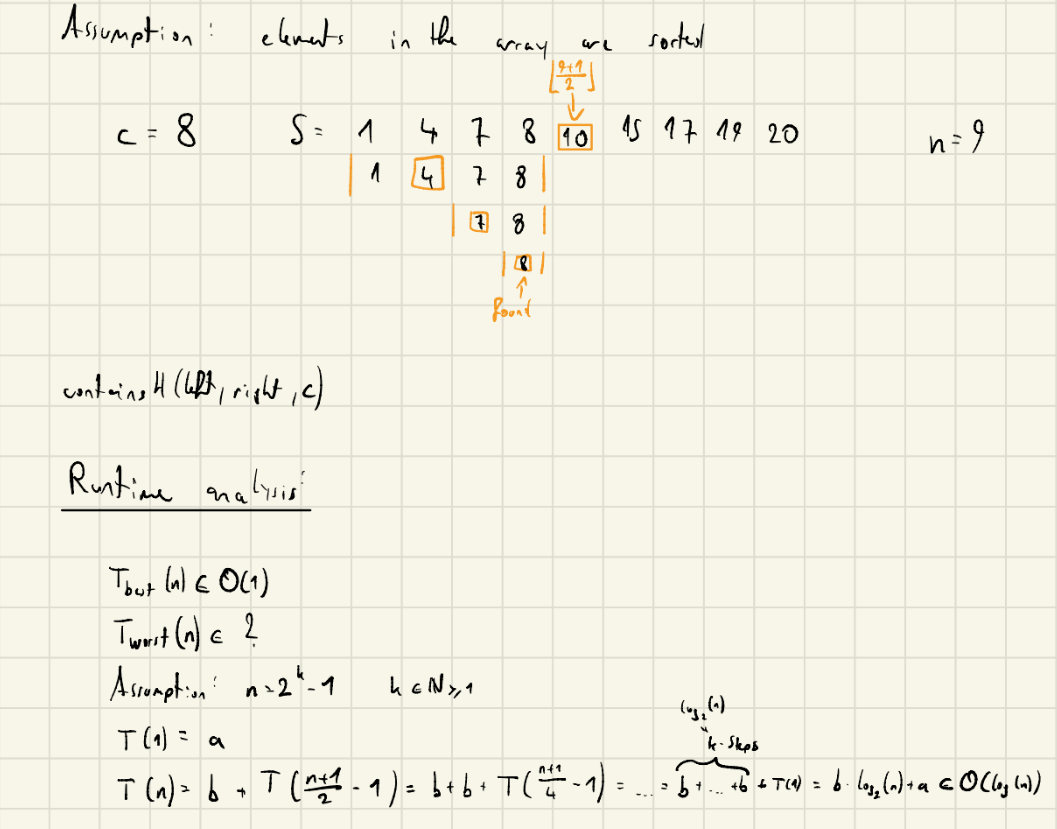
\includegraphics[scale = 0.4]{binary.png}
	
	The Binary search thus has a complexity of $\mathcal{O}(log_{2}(n))$ which in term is $\mathcal{O}(log(n))$. 
	
	For the complexity analysis of the Ternary search consider:
	
	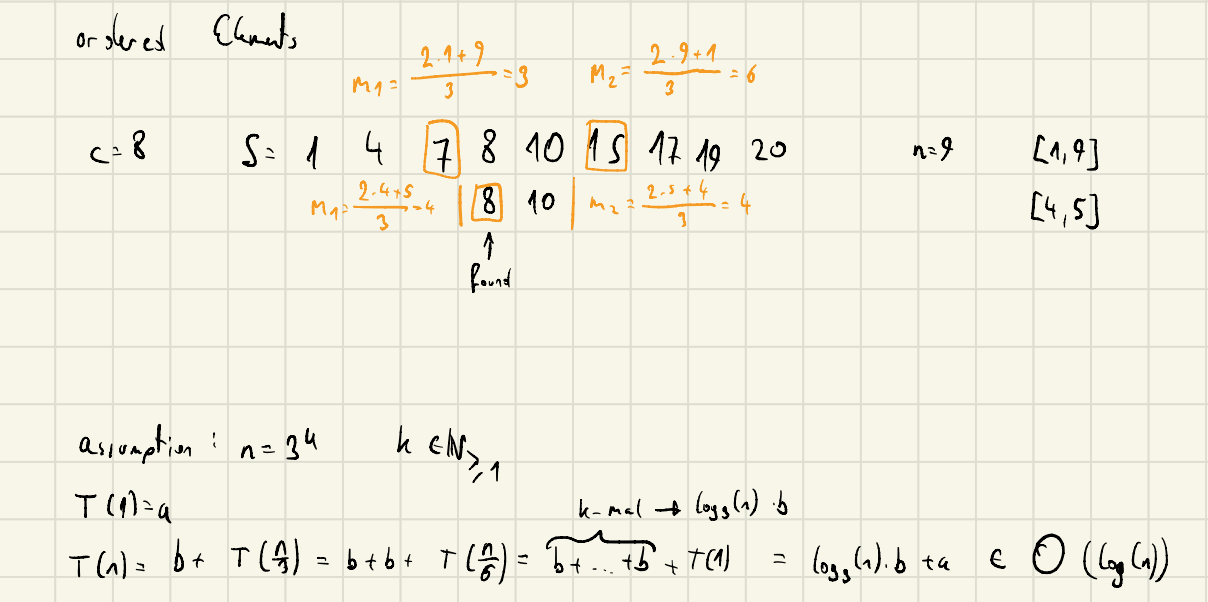
\includegraphics[scale = 0.3]{ternary.png}
	
	The Ternary search thus has a complexity of $\mathcal{O}(log_{3}(n))$ which in term is also $\mathcal{O}(log(n))$
	
	We conclude, that both concepts have the same order of complexity. Although the Binary search needs less comparisons, which makes it the more efficient variant in most cases.
	
	
\end{document}